\section{Análisis de Resultados}

En este capítulo se presentan y analizan los resultados obtenidos tras la implementación de Irakani Builder. Se evalúan aspectos funcionales, de rendimiento, integración de IA y la percepción de los usuarios finales mediante una encuesta de satisfacción.

\subsection{Resultados Funcionales}

\subsubsection{Módulos finalizados}

Durante el desarrollo del proyecto se completaron exitosamente los siguientes módulos principales:

\begin{itemize}
    \item \textbf{Sistema de autenticación y gestión de sesiones}: Implementación completa del login, registro y manejo de sesiones de usuario (Figura \ref{fig:ui_login}).
    
    \item \textbf{Selector de espacios y bases de datos}: Interfaz para la selección y gestión de espacios de trabajo y conexiones a bases de datos (Figuras \ref{fig:ui_space_selection} y \ref{fig:ui_access_selection}).
    
    \item \textbf{Editor visual de aplicaciones}: Panel principal con interfaz de arrastrar y soltar para la construcción de aplicaciones (Figura \ref{fig:ui_editor_visual}).
    
    \item \textbf{Sistema de paneles redimensionables}: Implementación de una interfaz flexible con paneles ajustables que mejora la experiencia de desarrollo (Figura \ref{fig:ui_redimensionable}).
    
    \item \textbf{Integración de Monaco Editor}: Editor de código profesional embebido en la plataforma web (Figura \ref{fig:ui_monaco_editor}).
    
    \item \textbf{Chat con IA}: Asistente inteligente para generación de código y resolución de dudas (Figura \ref{fig:ui_chat_ia}).
    
    \item \textbf{Generador automático de iconos}: Sistema de generación de iconos personalizados mediante IA (Figura \ref{fig:ui_generador_iconos}).
    
    \item \textbf{Sistema de notificaciones}: Implementación de notificaciones en tiempo real (Figura \ref{fig:ui_notificaciones}).
    
    \item \textbf{Gestión de temas}: Sistema de personalización visual de la plataforma (Figura \ref{fig:ui_temas}).
    
    \item \textbf{Administrador de base de datos}: Herramienta integrada para gestión de esquemas y datos (Figura \ref{fig:ui_db_admin}).
\end{itemize}

\textbf{Comparativa visual antes/después:}

La evolución de la plataforma representa un salto cualitativo significativo en términos de usabilidad y funcionalidad:

\textbf{Plataforma anterior (app.irakani.com):}
\begin{itemize}
    \item Aplicación web con framework obsoleto y limitaciones de compatibilidad
    \item Flujo de trabajo lineal y rígido
    \item Ausencia de asistencia inteligente
    \item Generación manual de componentes
    \item Editor de código básico
\end{itemize}

\textbf{Irakani Builder (actual):}
\begin{itemize}
    \item Plataforma web accesible desde cualquier dispositivo
    \item Interfaz modular con paneles redimensionables
    \item Asistente de IA integrado para generación de código y componentes
    \item Generación automática de iconos y formularios
    \item Monaco Editor profesional con autocompletado y sintaxis avanzada
    \item Sistema de preview en tiempo real
    \item Gestión visual de entidades, listas y perfiles
\end{itemize}

\subsubsection{Funcionamiento del Editor Visual y Chat con IA}

\textbf{Editor Visual:}

El editor visual constituye el núcleo de la plataforma, permitiendo a los usuarios construir aplicaciones mediante una interfaz intuitiva de arrastrar y soltar. Sus características principales incluyen:

\begin{itemize}
    \item \textbf{Panel de componentes}: Biblioteca de elementos predefinidos organizados por categorías (Figura \ref{fig:ui_panel_izquierdo}).
    
    \item \textbf{Área de diseño}: Canvas principal donde se ensamblan los componentes de la aplicación (Figura \ref{fig:ui_builder_completo}).
    
    \item \textbf{Panel de propiedades}: Configuración detallada de cada componente seleccionado (Figura \ref{fig:ui_propiedades}).
    
    \item \textbf{Vista de árbol}: Representación jerárquica de la estructura de la aplicación (Figura \ref{fig:ui_tree_view}).
    
    \item \textbf{Preview en tiempo real}: Visualización instantánea de los cambios realizados (Figura \ref{fig:ui_preview}).
\end{itemize}

\textbf{Chat con IA:}

El asistente de IA representa una innovación clave en la plataforma, proporcionando soporte inteligente durante todo el proceso de desarrollo. Sus capacidades incluyen:

\begin{itemize}
    \item \textbf{Generación de código}: Creación automática de funciones, componentes y lógica de negocio basada en descripciones en lenguaje natural.
    
    \item \textbf{Resolución de dudas}: Respuestas contextuales sobre sintaxis, mejores prácticas y uso de la plataforma.
    
    \item \textbf{Sugerencias de optimización}: Recomendaciones para mejorar el rendimiento y la estructura del código.
    
    \item \textbf{Generación de iconos}: Creación automática de iconos personalizados mediante prompts descriptivos (Figura \ref{fig:ui_flujo_generacion}).
    
    \item \textbf{Asistencia en componentes}: Generación y edición de componentes como listas, formularios, aplicaicones, perfiles, etc. 
\end{itemize}

El chat mantiene el contexto de la conversación y del proyecto actual, permitiendo interacciones más naturales y precisas. La integración con el editor permite aplicar directamente las sugerencias de la IA al código en desarrollo.

\subsection{Análisis de Rendimiento y Tiempos}

\subsubsection{Comparativa de tiempos de desarrollo}


Uno de los objetivos principales de Irakani Builder es reducir significativamente los tiempos de desarrollo de aplicaciones. Para evaluar este aspecto, se realizó una comparativa entre la plataforma anterior y la nueva versión.

\textbf{Resultados de la encuesta sobre ahorro de tiempo:}

Según los datos recopilados en la encuesta de satisfacción, los usuarios reportaron los siguientes niveles de ahorro de tiempo al crear prototipos básicos:

\begin{table}[h]
\centering
\begin{tabular}{|l|c|}
\hline
\textbf{Rango de ahorro de tiempo} & \textbf{Porcentaje de usuarios} \\
\hline
Más del 50\% & 33.3\% (1 usuario) \\
30 - 50\% & 66.7\% (2 usuarios) \\
\hline
\end{tabular}
\caption{Distribución de ahorro de tiempo reportado por usuarios}
\label{tab:ahorro-tiempo}
\end{table}

\begin{figure}[H]
\centering
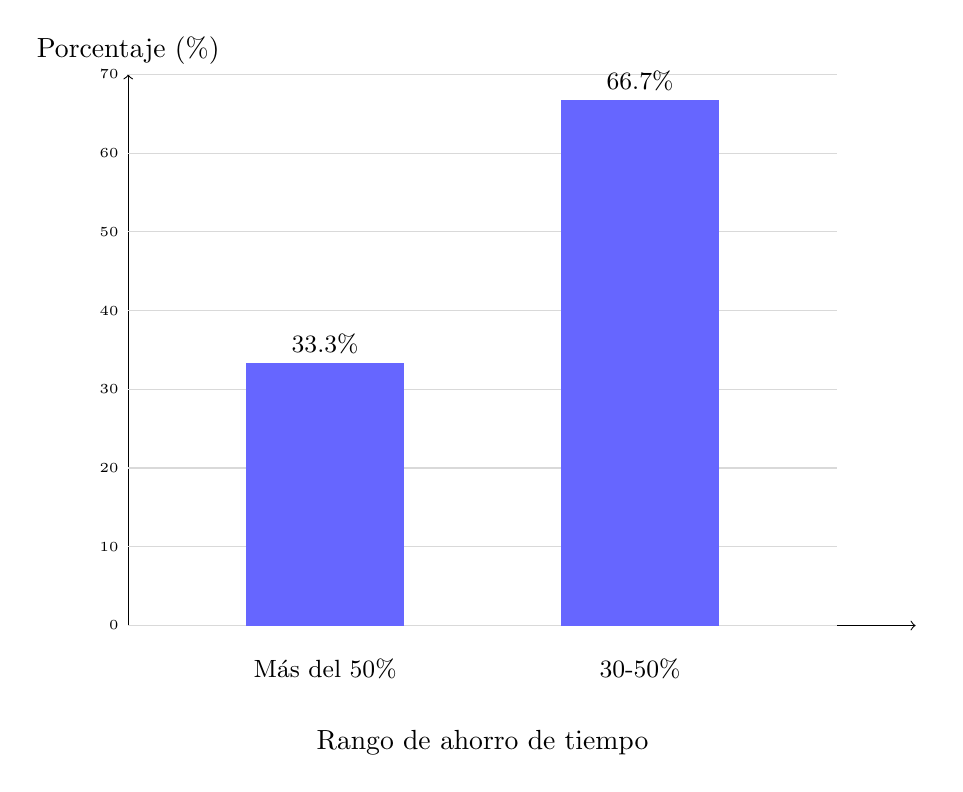
\begin{tikzpicture}[scale=1]
    % Ejes
    \draw[->] (0,0) -- (0,7) node[above] {Porcentaje (\%)};
    \draw[->] (0,0) -- (10,0) node[right] {};
    
    % Líneas de cuadrícula
    \foreach \y in {0,10,20,30,40,50,60,70} {
        \draw[gray!30] (0,\y/10) -- (9,\y/10);
        \node[left] at (0,\y/10) {\tiny \y};
    }
    
    % Barra 1: Más del 50%
    \fill[blue!60] (1.5,0) rectangle (3.5,3.33);
    \node[above] at (2.5,3.33) {\small 33.3\%};
    \node[below] at (2.5,-0.3) {\small Más del 50\%};
    
    % Barra 2: 30-50%
    \fill[blue!60] (5.5,0) rectangle (7.5,6.67);
    \node[above] at (6.5,6.67) {\small 66.7\%};
    \node[below] at (6.5,-0.3) {\small 30-50\%};
    
    \node[below] at (4.5,-1.2) {Rango de ahorro de tiempo};
\end{tikzpicture}
\caption{Distribución visual del ahorro de tiempo reportado}
\label{fig:ahorro-tiempo-grafico}
\end{figure}

Estos resultados indican que el 100\% de los usuarios encuestados perciben un ahorro de tiempo significativo (superior al 30\%), con un tercio de ellos reportando ahorros superiores al 50\%. Esto valida uno de los objetivos principales del proyecto: acelerar el proceso de desarrollo de aplicaciones.

\textbf{Factores que contribuyen al ahorro de tiempo:}

Los principales factores identificados que contribuyen a la reducción de tiempos son:

\begin{itemize}
    \item \textbf{Generación automática de código}: El asistente de IA reduce el tiempo de escritura manual de código repetitivo.
    
    \item \textbf{Generación de iconos y formularios}: La automatización de estos elementos elimina tareas tediosas y repetitivas.
    
    \item \textbf{Editor visual}: La interfaz de arrastrar y soltar acelera el prototipado inicial.
    
    \item \textbf{Preview en tiempo real}: La visualización instantánea reduce ciclos de prueba y error.
    
    \item \textbf{Integración de herramientas}: Tener todas las funcionalidades en una sola plataforma elimina cambios de contexto.
\end{itemize}

\subsubsection{Métricas de eficiencia operativa}

\textbf{Generación automática de componentes:}

La encuesta reveló que el 66.7\% de los usuarios considera que la generación automática de iconos y formularios acelera su flujo de trabajo de manera definitiva, mientras que el 33.3\% indica que lo hace parcialmente. Esto demuestra que las funcionalidades de automatización tienen un impacto positivo generalizado en la productividad.

\begin{figure}[H]
\centering
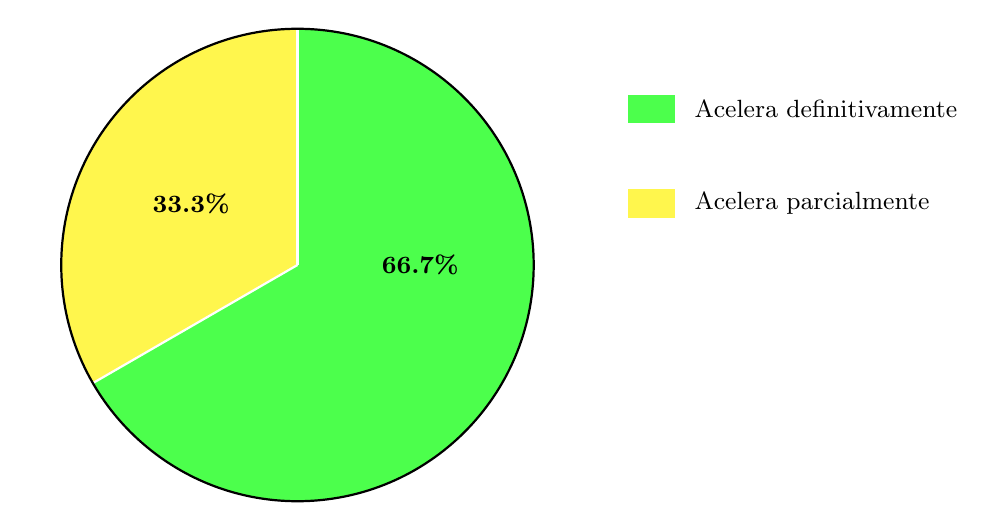
\begin{tikzpicture}[scale=1.2]
    % Gráfico de pastel
    \def\radius{2.5}
    
    % Segmento 1: 66.7% (240 grados)
    \fill[green!70] (0,0) -- (90:\radius) arc (90:-150:\radius) -- cycle;
    
    % Segmento 2: 33.3% (120 grados)
    \fill[yellow!70] (0,0) -- (-150:\radius) arc (-150:-270:\radius) -- cycle;
    
    % Líneas de separación
    \draw[white, thick] (0,0) -- (90:\radius);
    \draw[white, thick] (0,0) -- (-150:\radius);
    
    % Círculo exterior
    \draw[thick] (0,0) circle (\radius);
    
    % Etiquetas con porcentajes
    \node at (0:1.3) {\small \textbf{66.7\%}};
    \node at (-210:1.3) {\small \textbf{33.3\%}};
    
    % Leyenda
    \fill[green!70] (3.5,1.5) rectangle (4,1.8);
    \node[right] at (4.1,1.65) {\small Acelera definitivamente};
    
    \fill[yellow!70] (3.5,0.5) rectangle (4,0.8);
    \node[right] at (4.1,0.65) {\small Acelera parcialmente};
\end{tikzpicture}
\caption{Percepción del impacto de la generación automática en el flujo de trabajo}
\label{fig:generacion-automatica}
\end{figure}

\textbf{Utilidad del asistente de IA:}

En una escala del 1 al 5, la utilidad del asistente de IA para resolver dudas y generar código rápido obtuvo las siguientes calificaciones:

\begin{table}[h]
\centering
\begin{tabular}{|l|c|}
\hline
\textbf{Calificación} & \textbf{Número de usuarios} \\
\hline
5 (Muy útil) & 1 \\
4 (Útil) & 2 \\
\hline
\textbf{Promedio} & \textbf{4.33 / 5} \\
\hline
\end{tabular}
\caption{Evaluación de utilidad del asistente de IA}
\label{tab:utilidad-ia}
\end{table}

\begin{figure}[H]
\centering
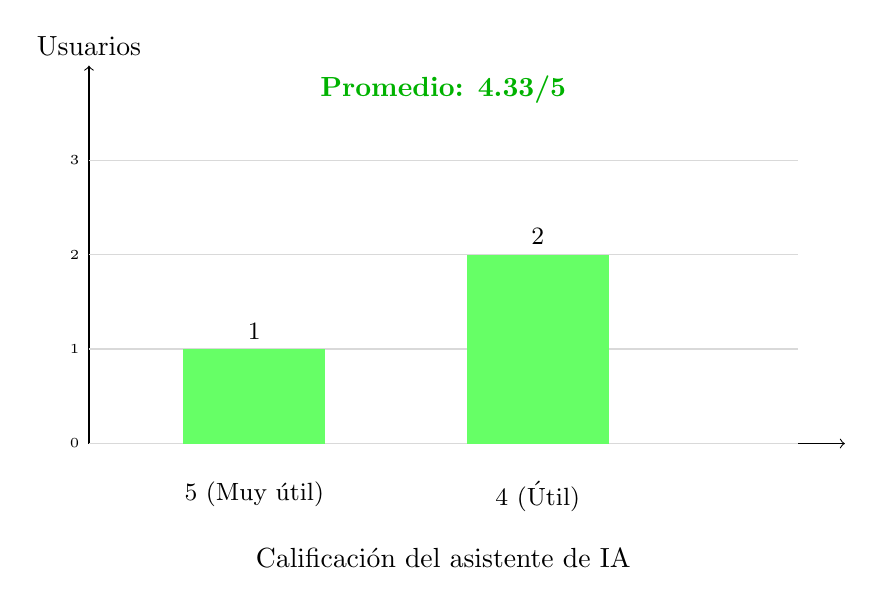
\begin{tikzpicture}[scale=1.2]
    % Ejes
    \draw[->] (0,0) -- (0,4) node[above] {Usuarios};
    \draw[->] (0,0) -- (8,0);
    
    % Líneas de cuadrícula
    \foreach \y in {0,1,2,3} {
        \draw[gray!30] (0,\y) -- (7.5,\y);
        \node[left] at (0,\y) {\tiny \y};
    }
    
    % Barra 1: Calificación 5
    \fill[green!60] (1,0) rectangle (2.5,1);
    \node[above] at (1.75,1) {\small 1};
    \node[below] at (1.75,-0.3) {\small 5 (Muy útil)};
    
    % Barra 2: Calificación 4
    \fill[green!60] (4,0) rectangle (5.5,2);
    \node[above] at (4.75,2) {\small 2};
    \node[below] at (4.75,-0.3) {\small 4 (Útil)};
    
    \node[below] at (3.75,-1) {Calificación del asistente de IA};
    \node[above, green!70!black, font=\bfseries] at (3.75,3.5) {Promedio: 4.33/5};
\end{tikzpicture}
\caption{Distribución de calificaciones del asistente de IA}
\label{fig:utilidad-ia-grafico}
\end{figure}

Con un promedio de 4.33 sobre 5, el asistente de IA es percibido como una herramienta altamente valiosa por los usuarios, validando la decisión de integrar capacidades de inteligencia artificial en la plataforma.

\subsection{Resultados de la Integración de IA}

\subsubsection{Precisión del código generado}

La calidad del código generado por la IA es un factor crítico para la adopción de la plataforma. Los usuarios evaluaron este aspecto considerando cuántas correcciones manuales requiere el código generado.

\textbf{Calificación de calidad del código:}

\begin{table}[h]
\centering
\begin{tabular}{|l|c|}
\hline
\textbf{Calificación} & \textbf{Número de usuarios} \\
\hline
4 (Buena calidad) & 1 \\
3 (Calidad aceptable) & 2 \\
\hline
\textbf{Promedio} & \textbf{3.33 / 5} \\
\hline
\end{tabular}
\caption{Calificación de calidad del código generado por IA}
\label{tab:calidad-codigo}
\end{table}

\begin{figure}[H]
\centering
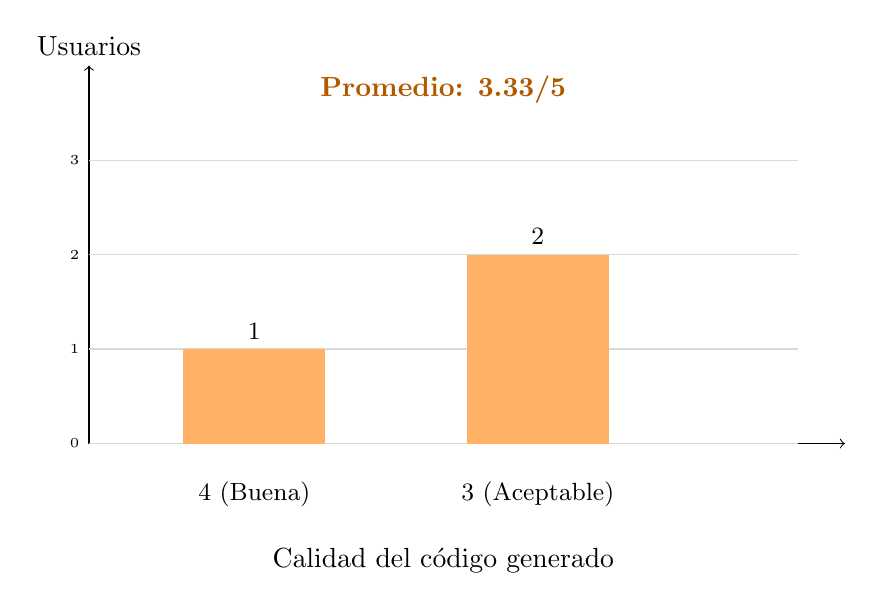
\begin{tikzpicture}[scale=1.2]
    % Ejes
    \draw[->] (0,0) -- (0,4) node[above] {Usuarios};
    \draw[->] (0,0) -- (8,0);
    
    % Líneas de cuadrícula
    \foreach \y in {0,1,2,3} {
        \draw[gray!30] (0,\y) -- (7.5,\y);
        \node[left] at (0,\y) {\tiny \y};
    }
    
    % Barra 1: Calificación 4
    \fill[orange!60] (1,0) rectangle (2.5,1);
    \node[above] at (1.75,1) {\small 1};
    \node[below] at (1.75,-0.3) {\small 4 (Buena)};
    
    % Barra 2: Calificación 3
    \fill[orange!60] (4,0) rectangle (5.5,2);
    \node[above] at (4.75,2) {\small 2};
    \node[below] at (4.75,-0.3) {\small 3 (Aceptable)};
    
    \node[below] at (3.75,-1) {Calidad del código generado};
    \node[above, orange!70!black, font=\bfseries] at (3.75,3.5) {Promedio: 3.33/5};
\end{tikzpicture}
\caption{Calidad del código generado por IA}
\label{fig:calidad-codigo-grafico}
\end{figure}

El promedio de 3.33 sobre 5 indica que el código generado es generalmente aceptable, aunque existe margen de mejora. Los usuarios reportan que el código requiere algunas correcciones manuales, pero no de manera excesiva.

\textbf{Frecuencia de alucinaciones:}

Un aspecto crítico en sistemas de IA generativa es la frecuencia con la que el modelo produce resultados incorrectos o alucinaciones. Los resultados de la encuesta son alentadores:

\begin{table}[h]
\centering
\begin{tabular}{|l|c|}
\hline
\textbf{Frecuencia de alucinaciones} & \textbf{Porcentaje} \\
\hline
Rara vez & 100\% (3 usuarios) \\
\hline
\end{tabular}
\caption{Frecuencia de alucinaciones o estructuras incorrectas generadas por IA}
\label{tab:alucinaciones}
\end{table}

El hecho de que el 100\% de los usuarios reporte que las alucinaciones ocurren rara vez es un indicador muy positivo de la fiabilidad del sistema de IA integrado. Esto sugiere que:

\begin{itemize}
    \item El contexto proporcionado a la IA es suficientemente específico
    \item Los prompts están bien diseñados
    \item El modelo seleccionado es apropiado para el dominio de aplicación
    \item Las validaciones implementadas son efectivas
\end{itemize}

\subsubsection{Análisis de costos y consumo de tokens}

La integración de IA mediante AWS Bedrock implica costos operativos que deben ser monitoreados y optimizados. Aunque no se recopilaron métricas específicas de consumo en la encuesta, es importante considerar los siguientes aspectos:

\textbf{Estrategias de optimización implementadas:}

\begin{itemize}    
    \item \textbf{Contexto selectivo}: Envío únicamente de la información relevante en cada consulta para minimizar tokens.
    
    \item \textbf{Límites de uso}: Implementación de cuotas por usuario para controlar costos.
    
    \item \textbf{Modelos diferenciados}: Uso de modelos más económicos para tareas simples y modelos avanzados solo cuando sea necesario.
\end{itemize}

\textbf{Proyección de costos:}

Basándose en el uso reportado y la frecuencia de interacciones con el asistente de IA, se estima que el costo promedio por usuario activo se mantiene dentro de rangos sostenibles para el modelo de negocio de la plataforma. La alta satisfacción con la funcionalidad (4.33/5) justifica la inversión en esta tecnología.

\subsection{Resultados de las Pruebas de Usuario}

Esta sección analiza en detalle las respuestas del cuestionario de satisfacción aplicado a los usuarios de Irakani Builder. La encuesta se diseñó para evaluar aspectos clave de la plataforma: eficiencia, productividad, calidad de la IA y usabilidad.

\subsubsection{Percepción de eficiencia y productividad}

\textbf{Ahorro de tiempo en desarrollo:}

Como se mencionó anteriormente, el 100\% de los usuarios reporta un ahorro de tiempo significativo:

\begin{itemize}
    \item 33.3\% ahorra más del 50\% del tiempo
    \item 66.7\% ahorra entre 30\% y 50\% del tiempo
\end{itemize}

Este resultado es especialmente relevante considerando que se trata de usuarios con experiencia en la plataforma anterior, lo que les permite hacer una comparación directa y fundamentada.

\textbf{Impacto de la automatización:}

La generación automática de iconos y formularios fue evaluada positivamente:

\begin{itemize}
    \item 66.7\% confirma que acelera definitivamente su flujo de trabajo
    \item 33.3\% indica que lo hace parcialmente
    \item 0\% reporta que no acelera el flujo de trabajo
\end{itemize}

Esto indica que las funcionalidades de automatización son efectivas y bien recibidas por la mayoría de los usuarios.

\subsubsection{Evaluación de calidad de la IA y Usabilidad}

\textbf{Calidad del asistente de IA:}

El asistente de IA obtuvo una calificación promedio de 4.33/5 en utilidad, con la siguiente distribución:

\begin{itemize}
    \item 33.3\% lo califica con 5 (máxima utilidad)
    \item 66.7\% lo califica con 4 (alta utilidad)
\end{itemize}

La calidad del código generado obtuvo un promedio de 3.33/5, lo que indica que:

\begin{itemize}
    \item El código es generalmente útil y funcional
    \item Requiere algunas correcciones manuales
    \item Existe espacio para mejoras en la precisión
\end{itemize}

La baja frecuencia de alucinaciones (100\% reporta rara vez) compensa parcialmente la calificación moderada de calidad, sugiriendo que cuando la IA genera código, este es mayormente correcto, aunque podría ser más refinado.

\textbf{Usabilidad de la interfaz:}

La interfaz de paneles redimensionables y el editor visual obtuvieron una calificación promedio de 3.33/5 en intuitividad:

\begin{table}[h]
\centering
\begin{tabular}{|l|c|}
\hline
\textbf{Calificación} & \textbf{Número de usuarios} \\
\hline
4 (Intuitiva) & 1 \\
3 (Moderadamente intuitiva) & 2 \\
\hline
\textbf{Promedio} & \textbf{3.33 / 5} \\
\hline
\end{tabular}
\caption{Evaluación de intuitividad de la interfaz}
\label{tab:intuitividad}
\end{table}

Este resultado sugiere que, aunque la interfaz es funcional, podría beneficiarse de mejoras en la experiencia de usuario para hacerla más intuitiva, especialmente para nuevos usuarios.

\textbf{Experiencia con Monaco Editor:}

La integración de Monaco Editor fue evaluada con un promedio de 3.67/5:

\begin{table}[h]
\centering
\begin{tabular}{|l|c|}
\hline
\textbf{Calificación} & \textbf{Número de usuarios} \\
\hline
4 (Buena experiencia) & 2 \\
3 (Experiencia aceptable) & 1 \\
\hline
\textbf{Promedio} & \textbf{3.67 / 5} \\
\hline
\end{tabular}
\caption{Evaluación de la experiencia con Monaco Editor}
\label{tab:monaco-editor}
\end{table}

Esta calificación indica que la integración del editor de código es bien recibida, aunque hay margen para optimizaciones en su implementación web.

\subsubsection{Interpretación global de la encuesta de satisfacción}

\textbf{Resumen de calificaciones:}

\begin{table}[h]
\centering
\begin{tabular}{|l|c|}
\hline
\textbf{Aspecto evaluado} & \textbf{Calificación promedio} \\
\hline
Utilidad del asistente de IA & 4.33 / 5 \\
Experiencia con Monaco Editor & 3.67 / 5 \\
Calidad del código generado & 3.33 / 5 \\
Intuitividad de la interfaz & 3.33 / 5 \\
\hline
\textbf{Promedio general} & \textbf{3.67 / 5} \\
\hline
\end{tabular}
\caption{Resumen de calificaciones de la encuesta}
\label{tab:resumen-calificaciones}
\end{table}

\begin{figure}[H]
\centering
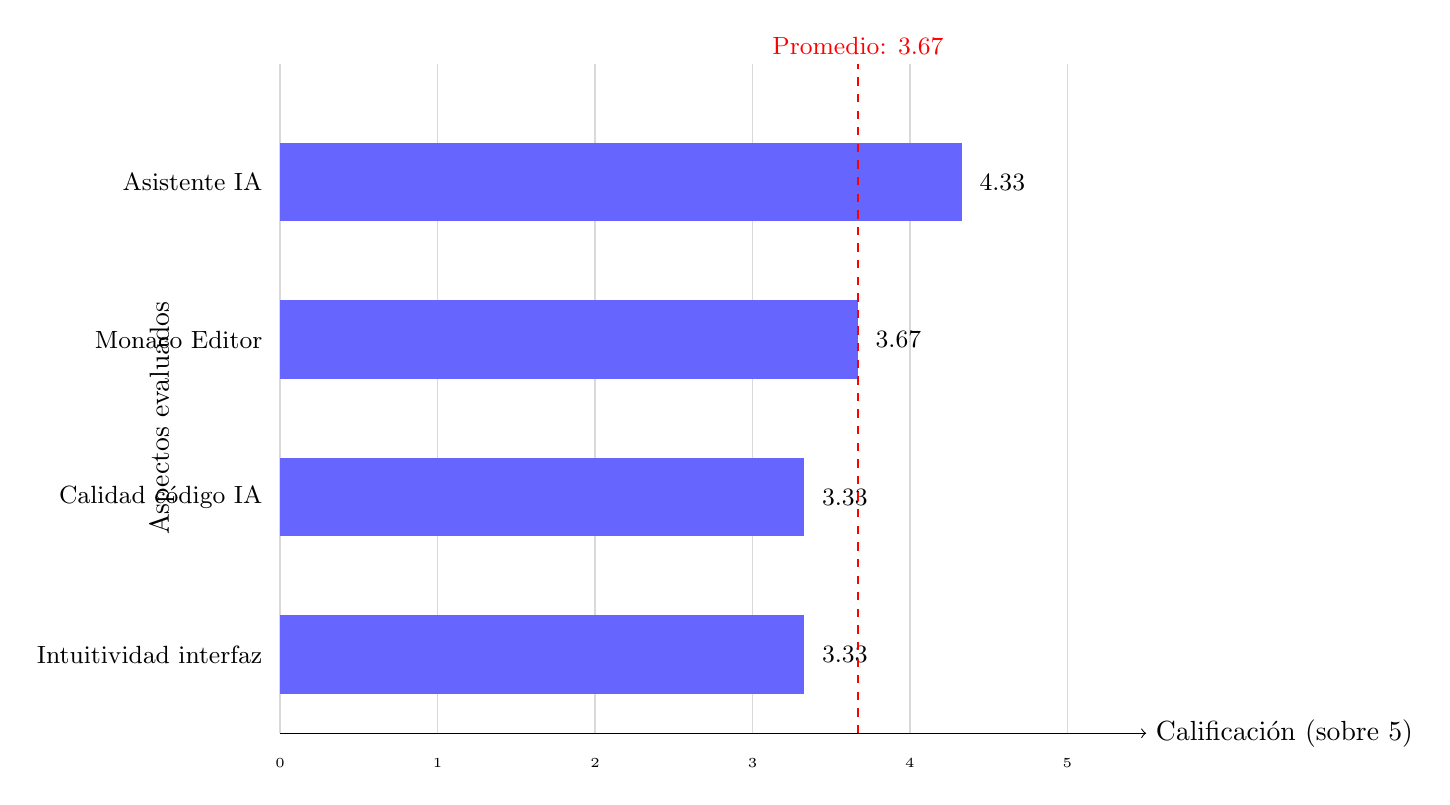
\begin{tikzpicture}[scale=1]
    % Título de eje Y
    \node[rotate=90] at (-1.5,4) {Aspectos evaluados};
    
    % Eje X
    \draw[->] (0,0) -- (11,0) node[right] {Calificación (sobre 5)};
    
    % Líneas de cuadrícula verticales
    \foreach \x in {0,1,2,3,4,5} {
        \draw[gray!30] (\x*2,0) -- (\x*2,8.5);
        \node[below] at (\x*2,-0.2) {\tiny \x};
    }
    
    % Barra 1: Intuitividad interfaz (3.33)
    \fill[blue!60] (0,0.5) rectangle (6.66,1.5);
    \node[right] at (6.76,1) {\small 3.33};
    \node[left] at (-0.1,1) {\small Intuitividad interfaz};
    
    % Barra 2: Calidad código IA (3.33)
    \fill[blue!60] (0,2.5) rectangle (6.66,3.5);
    \node[right] at (6.76,3) {\small 3.33};
    \node[left] at (-0.1,3) {\small Calidad código IA};
    
    % Barra 3: Monaco Editor (3.67)
    \fill[blue!60] (0,4.5) rectangle (7.34,5.5);
    \node[right] at (7.44,5) {\small 3.67};
    \node[left] at (-0.1,5) {\small Monaco Editor};
    
    % Barra 4: Asistente IA (4.33)
    \fill[blue!60] (0,6.5) rectangle (8.66,7.5);
    \node[right] at (8.76,7) {\small 4.33};
    \node[left] at (-0.1,7) {\small Asistente IA};
    
    % Línea de promedio
    \draw[red, dashed, thick] (7.34,0) -- (7.34,8.5);
    \node[red, above] at (7.34,8.5) {\small Promedio: 3.67};
\end{tikzpicture}
\caption{Comparativa de calificaciones por aspecto evaluado}
\label{fig:resumen-calificaciones-grafico}
\end{figure}

\textbf{Fortalezas identificadas:}

\begin{enumerate}
    \item \textbf{Asistente de IA}: Es la funcionalidad mejor valorada (4.33/5), demostrando que la integración de inteligencia artificial es un diferenciador clave de la plataforma.
    
    \item \textbf{Ahorro de tiempo}: El 100\% de usuarios reporta ahorros significativos (>30\%), validando el objetivo principal del proyecto.
    
    \item \textbf{Fiabilidad de la IA}: La baja frecuencia de alucinaciones genera confianza en el sistema.
    
    \item \textbf{Automatización}: La generación automática de componentes es valorada positivamente por todos los usuarios.
\end{enumerate}

\textbf{Áreas de mejora identificadas:}

\begin{enumerate}
    \item \textbf{Calidad del código generado}: Con 3.33/5, existe espacio para mejorar la precisión y reducir la necesidad de correcciones manuales.
    
    \item \textbf{Intuitividad de la interfaz}: La calificación de 3.33/5 sugiere que la curva de aprendizaje podría reducirse con mejoras en UX.
\end{enumerate}

\textbf{Sugerencias de los usuarios para versión 2.0:}

Los usuarios proporcionaron las siguientes sugerencias para futuras versiones:

\begin{itemize}
    \item \textbf{Duplicar espacios con IA}: Funcionalidad para clonar espacios de trabajo completos utilizando IA para adaptar el contenido.
    
    \item \textbf{Los indicadores pensando muy en futuro}: Mejora en el sistema de indicadores y métricas de la plataforma.
    
    \item \textbf{Crear y modificar indicadores de Irakani}: Herramientas más avanzadas para la gestión de indicadores y KPIs.
\end{itemize}

Estas sugerencias indican que los usuarios están pensando en casos de uso avanzados, lo cual es una señal positiva de adopción y compromiso con la plataforma.

\textbf{Conclusiones de la encuesta:}

La encuesta de satisfacción revela un balance positivo general:

\begin{itemize}
    \item La plataforma cumple su objetivo principal de reducir tiempos de desarrollo
    \item La integración de IA es altamente valorada y funciona de manera fiable
    \item Existen oportunidades claras de mejora en usabilidad y calidad del código generado
    \item Los usuarios están comprometidos y proponen mejoras constructivas
\end{itemize}

Con un promedio general de 3.67/5 y un 100\% de usuarios reportando ahorros significativos de tiempo, Irakani Builder demuestra ser una solución viable y efectiva para el desarrollo rápido de aplicaciones. Las áreas de mejora identificadas proporcionan una hoja de ruta clara para futuras iteraciones del producto.

\begin{figure}[H]
\centering
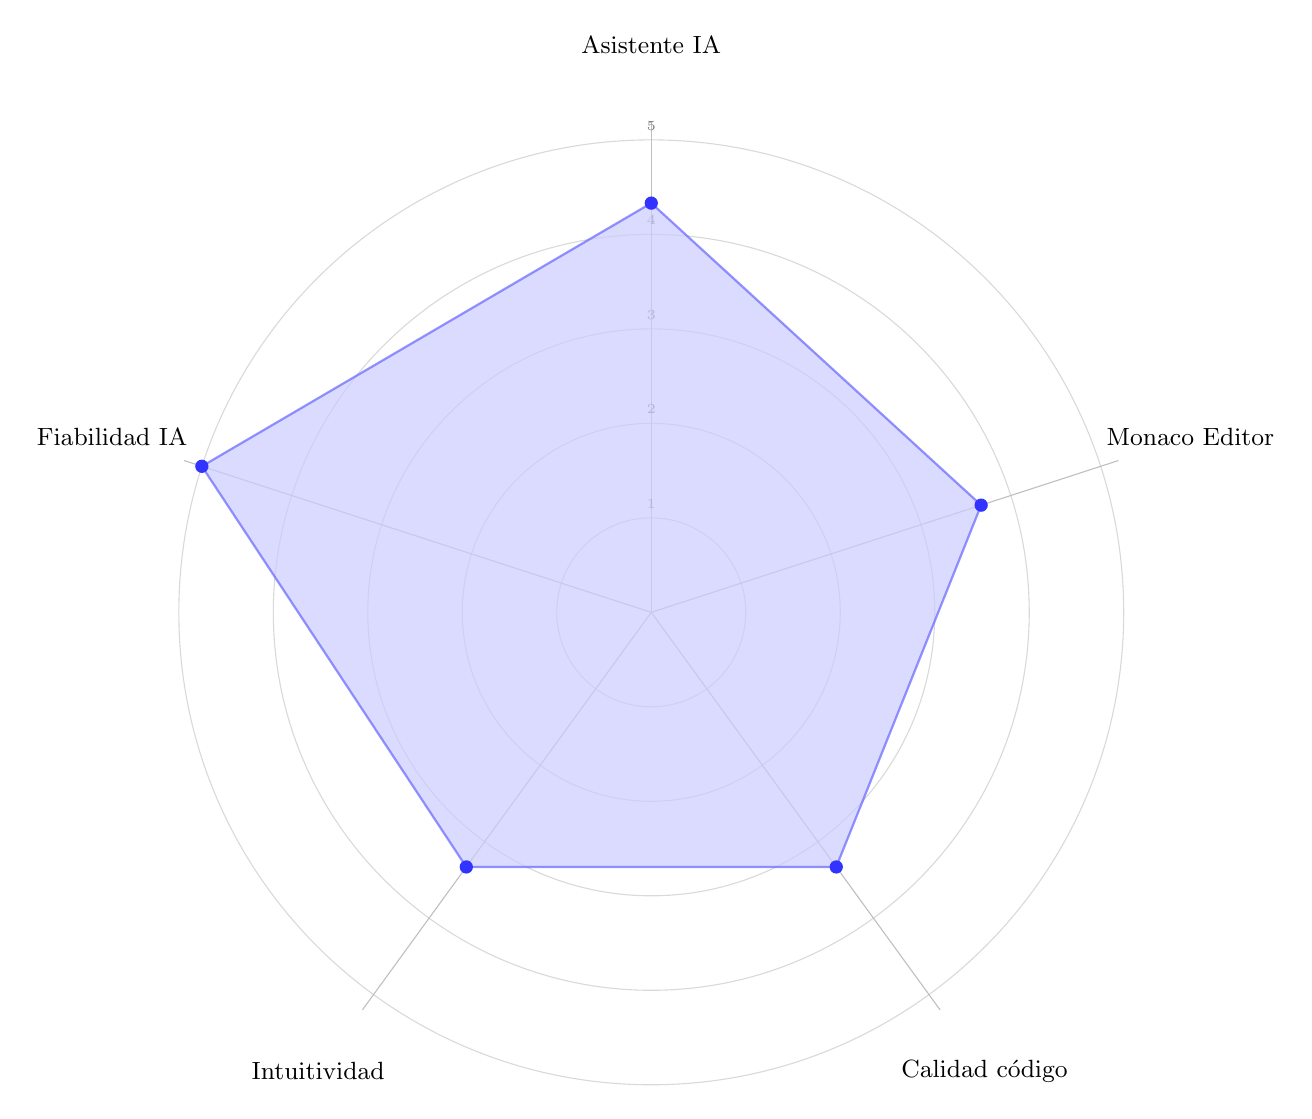
\begin{tikzpicture}[scale=1.2]
    % Círculos de referencia
    \foreach \r in {1,2,3,4,5} {
        \draw[gray!30] (0,0) circle (\r cm);
    }
    
    % Líneas radiales y etiquetas
    \foreach \angle/\label in {
        90/Asistente IA,
        18/Monaco Editor,
        -54/Calidad código,
        -126/Intuitividad,
        -198/Fiabilidad IA
    } {
        \draw[gray!50] (0,0) -- (\angle:5.2cm);
        \node at (\angle:6cm) {\small \label};
    }
    
    % Etiquetas de escala
    \foreach \r/\val in {1/1, 2/2, 3/3, 4/4, 5/5} {
        \node[gray, font=\tiny] at (90:\r cm) [anchor=south] {\val};
    }
    
    % Datos (normalizados a escala de 5)
    \coordinate (A) at (90:4.33cm);    % Asistente IA: 4.33
    \coordinate (B) at (18:3.67cm);    % Monaco Editor: 3.67
    \coordinate (C) at (-54:3.33cm);   % Calidad código: 3.33
    \coordinate (D) at (-126:3.33cm);  % Intuitividad: 3.33
    \coordinate (E) at (-198:5cm);     % Fiabilidad IA: 5 (100% rara vez alucinaciones)
    
    % Polígono de datos
    \draw[blue!60, fill=blue!20, thick, opacity=0.7] 
        (A) -- (B) -- (C) -- (D) -- (E) -- cycle;
    
    % Puntos de datos
    \foreach \point in {A,B,C,D,E} {
        \fill[blue!80] (\point) circle (2pt);
    }
\end{tikzpicture}
\caption{Perfil de evaluación de Irakani Builder (escala 1-5)}
\label{fig:radar-evaluacion}
\end{figure}
